\documentclass[
a4paper,
oneside,
10pt,
fleqn,
headsepline,
toc=listofnumbered, 
bibliography=totocnumbered]{scrartcl}

% deutsche Trennmuster etc.
\usepackage[T1]{fontenc}
\usepackage[utf8]{inputenc}
\usepackage[english, ngerman]{babel} % \selectlanguage{english} if  needed
\usepackage{lmodern} % use modern latin fonts

% Custom commands
\newcommand{\AUTHOR}{Michael Wieland}
\newcommand{\SECONDAUTHOR}{Fabian Hauser}
\newcommand{\INSTITUTE}{Hochschule für Technik Rapperswil}
\newcommand{\GITHUB}{https://github.com/michiwieland/hsr-zusammenfassungen}
\newcommand{\LICENSEURL}{https://www.gnu.org/licenses/gpl-3.0.de.html}
\newcommand{\LICENSE}{https://www.gnu.org/licenses/gpl-3.0.de.html}

% Jede Überschrift 1 auf neuer Seite
\let\stdsection\section
\renewcommand\section{\clearpage\stdsection}

% Multiple Authors
\usepackage{authblk}

% Layout / Seitenränder
\usepackage{geometry}

% Inhaltsverzeichnis
\usepackage{makeidx} 
\makeindex

\usepackage{url}
\usepackage[pdfborder={0 0 0}]{hyperref}
\usepackage[all]{hypcap}
\usepackage{hyperxmp} % for license metadata

% Glossar und Abkürzungsverzeichnis
\usepackage[acronym,toc,nopostdot]{glossaries}
\glossarystyle{altlisthypergroup}
\usepackage{xparse}
\DeclareDocumentCommand{\newdualentry}{ O{} O{} m m m m } {
	\newglossaryentry{gls-#3}{name={#5},text={#5\glsadd{#3}},
		description={#6},#1
	}
	\makeglossaries
	\newacronym[see={[Siehe:]{gls-#3}},#2]{#3}{#4}{#5\glsadd{gls-#3}}
}
\makeglossaries

% Mathematik
\usepackage{amsmath}
\usepackage{amssymb}
\usepackage{amsfonts}
\usepackage{enumitem}

% Images
\usepackage{graphicx}
\graphicspath{{images/}} % default paths

% Boxes
\usepackage{fancybox}

%Tables
\usepackage{tabu}
\usepackage{booktabs} % toprule, midrule, bottomrule
\usepackage{array} % for matrix tables

% Multi Columns
\usepackage{multicol}

% Header and footer
\usepackage{scrlayer-scrpage}
\setkomafont{pagehead}{\normalfont}
\setkomafont{pagefoot}{\normalfont}
\automark*{section}
\clearpairofpagestyles
\ihead{\headmark}
\ohead{\TITLE}
\cfoot{\pagemark}

% Pseudocode
\usepackage{algorithm}
\usepackage{algorithmic}

% Code Listings
\usepackage{listings}
\usepackage{color}
\usepackage{beramono}

\definecolor{DarkPurple}{rgb}{0.4, 0.1, 0.4}
\definecolor{DarkCyan}{rgb}{0.0, 0.5, 0.4}
\definecolor{LightLime}{rgb}{0.3, 0.5, 0.4}
\definecolor{Blue}{rgb}{0.0, 0.0, 1.0}

\lstdefinestyle{eclipse-style}{
	language=Java,  
	columns=flexible,
	showstringspaces=false,     
	basicstyle=\footnotesize\ttfamily, 
	keywordstyle=\bfseries\color{DarkPurple},
	commentstyle=\color{LightLime},
	stringstyle=\color{Blue}, 
	escapeinside={£}{£}, % latex scope within code      
	morekeywords={length},
	numbers=left,
	numberstyle=\tiny\color{black},
	frame=single,
}
\lstset{style=eclipse-style}


% Theorems \begin{mytheo}{title}{label}
\usepackage{tcolorbox}
\tcbuselibrary{theorems}
\newtcbtheorem[number within=section]{definiton}{Definition}%
{fonttitle=\bfseries}{def}
\newtcbtheorem[number within=section]{remember}{Merke}%
{fonttitle=\bfseries}{rem}

% Dokumentinformationen
\newcommand{\SUBJECT}{Dokumentation}
\newcommand{\TITLE}{Sunrise Clock}

% pdf metadata
\hypersetup{
	pdfauthor={\AUTHOR},
	pdftitle={\SUBJECT \TITLE},
	pdfcopyright={\LICENSE},
	pdflicenseurl={\LICENSEURL}
}

\begin{document}
	
% Front page
\title{\TITLE}
\subject{\SUBJECT}
\author{\SECONDAUTHOR}
\author{\AUTHOR}
\affil{\INSTITUTE}
\date{\today}
\maketitle

\vfill

% Licence
\paragraph{Lizenz} \hfill \\
\LICENSE

% Table of contents
\tableofcontents


% Glossar and acronyms (if included \loadglsentries{glossar})
\printglossary[type=\acronymtype]
\printglossary
\glsaddall


\section{Vorbereitung}

\subsection{Einleitung}
Das Projekt enstand aus der Idee heraus, leichter aufzuwachen, wenn es am Vorabend wieder einmal ein wenig später geworden ist. Die von uns verwendete Mi-Light Lampe lässt sich im 2.4GHz Funknetz mit fix definierten Befehlen ansprechen. Zur Steuerung der Lampe verwenden wir den kompakten Raspberry Pi Zero, auf welchem eine einfache NodeJS Applikation läuft, mit welcher die Weck-Konfigurationen verwaltet werden können. Das Frontend kann einfach über das Smartphone angesprochen werden. Einmal konfiguriert weckt einem die Sunrise Clock langsam wie beim Sonnenaufgang.

\subsection{Hardware}
Was du für deinen persönliche Sunrise Clock benötigst:
\begin{itemize}
	\item Raspberry Pi Zero mit 
	\begin{itemize}
		\item Raspberry Pi WiFi dongle
		\item micro-B USB Ladekabel um den Raspberry Pi Zero mit Strom zu versorgen
		\item microSD Karte
		\item Dupont cable (auf beiden Seiten female) für die Verbindung zwischen Wireless Sender und Raspberry Pi Zero
	\end{itemize}
	\item nRF24L01+ 2.4Ghz Wireless Sender \footnote{http://www.dx.com/de/p/nrf24l01-2-4ghz-wireless-transceiver-module-black-149483}
	\item Mi-Light GU10 Wireless Lamp 
	\item Mi-Light Remote (optional)
\end{itemize}

\begin{figure}[h]
	\centering
	\begin{minipage}[t]{0.3\textwidth}
		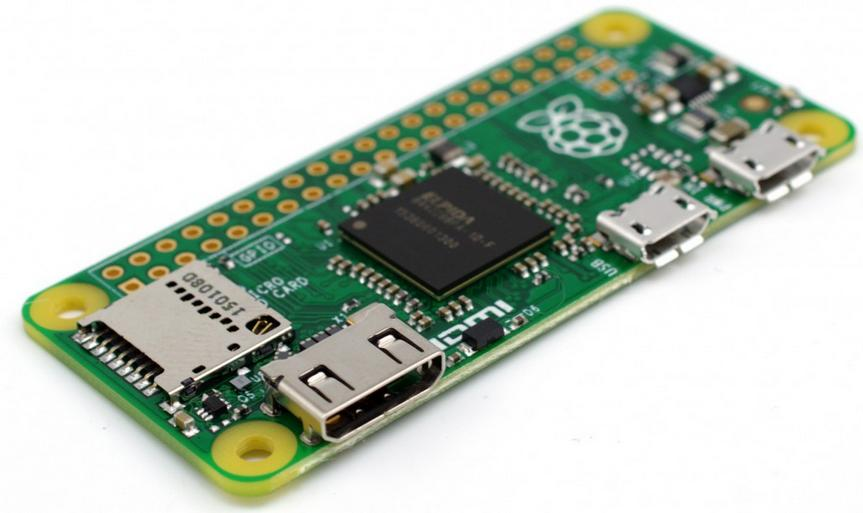
\includegraphics[width=\textwidth]{raspberry_zero}
		\caption{Raspberry Pi Zero}
	\end{minipage}
	\hfill
	\begin{minipage}[t]{0.3\textwidth}
		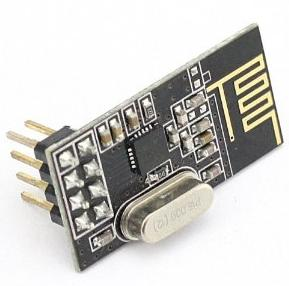
\includegraphics[width=\textwidth]{nrf24l01}
		\caption{nRF24L01+}
	\end{minipage}
	\begin{minipage}[t]{0.3\textwidth}
		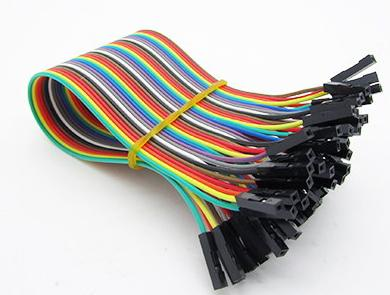
\includegraphics[width=\linewidth]{dupont_female}
		\caption{Dupont Kabel (2x weiblich)}
	\end{minipage}
\end{figure}


\subsection{Funktchip verbinden}
Der nRF24L01+ Funkchip wird nun mit den weiblichen Dupont Kabel mit dem Raspberry Pi Zero verbunden. Dazu kann der Pin-Belegungs-Plan \footnote{http://pinout.xyz} nützlich sein. Der Funkchip kann im 2.4 GHz Bereich von 2400MHz bis über 25000Mhz mit 1Mhz Kanalabstand senden und emfangen. Das Mi-Light Protokoll benutzt die drei Frequenzen 2411Mhz, 2442MHz und 2473MHz. 
\begin{table}[h]
\centering
\begin{tabu} to \linewidth {l c c}
	\toprule
	Leitung & Pim beim nRF24L01+ & Pin beim Raspberry Pi Zero \\
	GND (Ground / Erdung) & 1 & 20 \\
	3.3 Volt & 2 & 17 \\
	CE (chip enable bzw. slave select) & 3 & 22 \\
	CSN (chip select not) & 4 & 24 \\
	SCLK (serial clock) & 5 & 23 \\ 
	MOSI (Master Output Slave Input) & 6 & 19 \\
	MISO (Master Input Slave Output) & 7 & 21 \\
	\bottomrule
	\end{tabu}
	\caption{Dupont Verbindungen zwischen Raspberry Pi Zero und nRF24L01+}
\end{table}


\subsection{Raspberry im Headless Mode aufsetzen}
Der Headless Mode bedeutet, dass der Raspberry Pi nur über einen SSH Terminal konfiguriert, und auf eine grafische Oberfläche verzichtet wird. Diese wir für unser Projekt nämlich gar nicht benötigt.

\subsubsection{Rasbian herunterladen}
\begin{hint}{Partitionsnummer}{}
Für das kopieren des Rasbian mittels \lstinline|dd| muss die Partitionsnummer unbedingt weggelassen werden. Beim unmounten mittels \lstinline|dd| ist sie hingegen zwingend nötig. Zur Erinnerung. Die Partitionsnummer ist die Zahl ganz am Schluss des Dateisystem-Names (z.B \lstinline|/dev/sdx1|)
\end{hint}
\begin{enumerate}
	\item SD Karte mit dem Notebook verbinden
	\item Das aktuelle Rasbian ISO Image herunterladen \footnote{https://www.raspberrypi.org/downloads/raspbian/}
	\item Mit \lstinline|df -h| die SD Karte identifizieren. Die Karte wird wahrscheinlich als \lstinline|/dev/sdxx1| aufgelistet werden. Die Zahl im Gerätename ist die Partitionsnummer. Da wir das ISO Image aber auf die komplette Karte schreiben wollen, lassen wir die Zahl einfach weg. 
	\item Nun muss die Karte mit \lstinline|umount /dev/sdxx1| unmounted werden. Für diesen Befehl muss die Partitionsnummer verwendet werden
	\item Nun kann das Image auf die Karte kopiert werden. Es ist enorm wichtig dass du das korrekte Geräte als Ziel angibt. Ansonsten überschreibst du allenfalls die eigene Platte und das ist nicht unser Ziel. Führe also folgenden Befehl aus und passe ihn gegebenfalls für dein System an:
	\item \lstinline|sudo dd bs=4M if=/tmp/path/to/my/raspian.img of=/dev/sdxx|. WICHTIG: Hier muss die Partitions Nummer weggelassen werden
	\item Dies kann eine Weile dauern. Mit ein wenig Geduld beendet der Prozess aber und man kann mit dem nächsten Schritt weiterfahren.
	\item Mit dem Befehl \lstinline|sync| wird der Zwischenspeicher nochmals geleert.
	\item Nun ist Rasbian auf die SD Karte kopiert. Die SD Karte muss nun wieder gemounted werden. Am einfachsten geht dies indem man die Karte einmal herauszieht und wieder einfügt. 
	\item Nun muss geprüft werden wo die Karte gemounted wurde. Dies geht mit dem Befehl \lstinline|df -h|
	\item Der Mount Point für deine SD Karte liegt nur vermutlich irgendwo unter \lstinline|/run/media/[user]/[xxxx]|
	\item Wechsele nun in genau dieses Verzeichnis mittels \lstinline|cd|. Du bist nun auf der SD Karte und kannst die Files des Rasbian anpassen.
\end{enumerate}

\subsubsection{Wireless konfigurieren}
\begin{remember}{Korrekter Ordner}{}
Beachte bei den folgenden Schritten stets, dass du dich im Ordner auf der SD Karte und nicht in einem gleichbenannten Ordner deines Systems befindest. (z.B /etc/network $\Rightarrow$ System, etc/network $\Rightarrow$ Raspberry Pi Zero)
\end{remember}
\begin{enumerate}
	\item Wechsle wie oben erwähnt in den Ordner des gemounteten Rasbian und öffne das Wireless Konfigurations File mit folgendem Befehl
	\item Öffne \lstinline|sudo vim ./etc/network/interfaces| und vervollständige den vorhanden Eintrag mit dem Folgenden. 
\begin{lstlisting}[caption=/etc/network/interfaces]
auto wlan0
allow-hotplug wlan0
iface wlan0 inet manual
	address 192.168.1.20 # ip of your raspberry zero
	netmask 255.255.255.0
	gateway 192.168.1.1 # ip of your router
	wpa-conf /etc/wpa\_supplicant/wpa\_supplicant.conf
\end{lstlisting}
	\item Optional können noch die DNS Server von Google eingefügt werden. \lstinline|vim ./etc/resolve.conf|
\begin{lstlisting}[caption=/etc/resolve.conf]
# Google nameservers
nameserver 8.8.8.8
nameserver 8.8.4.4
\end{lstlisting}
	\item \lstinline|sudo vim ./etc/wpa\_supplicant/wpa\_supplicant.conf|
\begin{lstlisting}[caption=/etc/wpa\_supplicant/wpa\_supplicant.conf]
network={
	ssid="your wlan ssid"
	psk="your password"
	proto=RSN
	key_mgmt=WPA-PSK
	scan_ssid=1
}
\end{lstlisting}
	\item Die SD Karte mit dem Rasbian ist nun betriebsbereit und kann aus deinen persönlichen System ausgesteckt und beim Raspberry Pi Zero eingesteckt werden. Vor dem ausstecken sollte folgender Befehl ausgeführt werden: \lstinline|umount /run/media/[user]/[xxxx]|
\end{enumerate}

\subsubsection{Verbinden}
Stelle sicher dass der WLAN Dongle und die SD Karte im Raspberry Pi Zero angeschlossen ist. Danach kann der Raspberry Pi mit dem Strom verbunden werden. Wenn du alles vorgehende richtig gemacht hast, booted der Raspberry innerhalb von 30-45s.
\begin{enumerate}
	\item ssh pi@192.168.1.20
	\item Passwort eingeben (default ist \lstinline|raspberry|)
\end{enumerate}

\subsubsection{Rasbian konfigurieren}
%TODO Config Mode
\begin{lstlisting}
sudo apt-get update -y
sudo apt-get upgrade -y
sudo apt-get dist-upgrade -y
sudo raspi-config
\end{lstlisting}

\subsubsection{Git installieren}
Unser Projekt mit dem NodeJS Server und den benötigten Libraries ist frei auf Github verfügbar. Damit wir das Projekt auf den Raspberry Pi klonen können, benötigen wird \lstinline|git|
\begin{lstlisting}[caption=Git installieren]
sudo apt-get install git
\end{lstlisting}

\subsubsection{Node installieren}
Wie bereits erwähnt setzen wir auf eine einfach Node JS Applikation. 
\begin{lstlisting}[caption=Node installieren]
wget https://nodejs.org/dist/latest-v4.x/node-v4.5.0-linux-armv6l.tar.gz   
tar -xvf node-v4.3.2-linux-armv6l.tar.gz 
cd node-v4.3.2-linux-armv6l
sudo cp -R * /usr/local/
\end{lstlisting}

\subsection{Github Project klonen}
\begin{lstlisting}[caption=Github klonen]
git clone https://github.com/michiwieland/sunrise-clock
cd sunrise-clock
make all
sudo make install	
\end{lstlisting}

\section{Befehle}
\begin{itemize}
	\item Die ersten 3 Byte eines Befehls gehören zum Remote und könnnen per Brute Force herausgefunden oder vom gekauften Remote mit Wireshark gensnifft werden.
	\item Das 4te Byte ist die Farbe
	\item Das 5te Byte ist die Helligkeit
	\item Das 6te byte ist der Knopf beim Remote
	\item Das 7te und damit letzte Byte ist die Sequenz Nummer
\end{itemize}

\begin{table}[h]
	\centering
	\begin{tabu} to \linewidth {l l}
		\toprule
		Hexwert & Taste \\
		0x01 & alle LED Gruppen einschalten \\
		0x02 & alle LED Gruppen ausschalten \\
		0x03 & LED Gruppe 1 einschalten \\
		0x04 & LED Gruppe 1 ausschalten \\
		0x05 & LED Gruppe 2 einschalten \\
		0x06 & LED Gruppe 2 ausschalten \\
		0x07 & LED Gruppe 3 einschalten \\
		0x08 & LED Gruppe 3 ausschalten \\
		0x08 & LED Gruppe 4 einschalten \\
		0x09 & LED Gruppe 4 ausschalten \\
		0x0E & Slider für die Helligkeit \\
		
		\bottomrule
	\end{tabu}
	\caption{Openmilight Hex Befehlstabelle}
\end{table}




\appendix

% Code Listings
\lstlistoflistings

% List of figures
\listoffigures

% List of tables
\listoftables

% Bibliography
\bibliographystyle{plain} 
\bibliography{literatur}

\end{document}